\documentclass[]{article}
\usepackage{lmodern}
\usepackage{amssymb,amsmath}
\usepackage{ifxetex,ifluatex}
\usepackage{fixltx2e} % provides \textsubscript
\ifnum 0\ifxetex 1\fi\ifluatex 1\fi=0 % if pdftex
  \usepackage[T1]{fontenc}
  \usepackage[utf8]{inputenc}
\else % if luatex or xelatex
  \ifxetex
    \usepackage{mathspec}
  \else
    \usepackage{fontspec}
  \fi
  \defaultfontfeatures{Ligatures=TeX,Scale=MatchLowercase}
\fi
% use upquote if available, for straight quotes in verbatim environments
\IfFileExists{upquote.sty}{\usepackage{upquote}}{}
% use microtype if available
\IfFileExists{microtype.sty}{%
\usepackage{microtype}
\UseMicrotypeSet[protrusion]{basicmath} % disable protrusion for tt fonts
}{}
\usepackage[b5paper,tmargin=2.5cm,bmargin=2.5cm,lmargin=3.5cm,rmargin=2.5cm]{geometry}
\usepackage{hyperref}
\hypersetup{unicode=true,
            pdftitle={Big Brother Is Watching : Using Digital Surveillance Tools for Near Real-Time Mapping of the Risk of International Infectious Disease Spread},
            pdfauthor={Sangeeta Bhatia, Anne Cori and Pierre Nouvellet},
            pdfborder={0 0 0},
            breaklinks=true}
\urlstyle{same}  % don't use monospace font for urls
\usepackage{longtable,booktabs}
\usepackage{graphicx,grffile}
\makeatletter
\def\maxwidth{\ifdim\Gin@nat@width>\linewidth\linewidth\else\Gin@nat@width\fi}
\def\maxheight{\ifdim\Gin@nat@height>\textheight\textheight\else\Gin@nat@height\fi}
\makeatother
% Scale images if necessary, so that they will not overflow the page
% margins by default, and it is still possible to overwrite the defaults
% using explicit options in \includegraphics[width, height, ...]{}
\setkeys{Gin}{width=\maxwidth,height=\maxheight,keepaspectratio}
\IfFileExists{parskip.sty}{%
\usepackage{parskip}
}{% else
\setlength{\parindent}{0pt}
\setlength{\parskip}{6pt plus 2pt minus 1pt}
}
\setlength{\emergencystretch}{3em}  % prevent overfull lines
\providecommand{\tightlist}{%
  \setlength{\itemsep}{0pt}\setlength{\parskip}{0pt}}
\setcounter{secnumdepth}{5}
% Redefines (sub)paragraphs to behave more like sections
\ifx\paragraph\undefined\else
\let\oldparagraph\paragraph
\renewcommand{\paragraph}[1]{\oldparagraph{#1}\mbox{}}
\fi
\ifx\subparagraph\undefined\else
\let\oldsubparagraph\subparagraph
\renewcommand{\subparagraph}[1]{\oldsubparagraph{#1}\mbox{}}
\fi

%%% Use protect on footnotes to avoid problems with footnotes in titles
\let\rmarkdownfootnote\footnote%
\def\footnote{\protect\rmarkdownfootnote}

%%% Change title format to be more compact
\usepackage{titling}

% Create subtitle command for use in maketitle
\newcommand{\subtitle}[1]{
  \posttitle{
    \begin{center}\large#1\end{center}
    }
}

\setlength{\droptitle}{-2em}
  \title{Big Brother Is Watching : Using Digital Surveillance Tools for Near
Real-Time Mapping of the Risk of International Infectious Disease Spread}
  \pretitle{\vspace{\droptitle}\centering\huge}
  \posttitle{\par}
  \author{Sangeeta Bhatia, Anne Cori and Pierre Nouvellet}
  \preauthor{\centering\large\emph}
  \postauthor{\par}
  \date{}
  \predate{}\postdate{}


\begin{document}
\maketitle

In our increasingly interconnected world, it is crucial to understand
the risk of an outbreak originating in one country/region and spreading
to the rest of the world. Rapid recognition and response to potential
pandemics and emerging diseases have become essential global health
priorities. Digital disease surveillance tools such as ProMed and
HealthMap have the potential to serve as important early warning systems
as well as complement the field surveillance data during an ongoing
outbreak. While there are a number of systems that carry out digital
disease surveillance, there is as yet a lack of tools that can compile
and analyse the generated data to produce easily understood actionable
reports. We present a flexible statistical model that uses different
streams of data (such as disease surveillance data, mobility data etc.)
for short-term incidence trend forecasting.\\
In validating the model using data collected by ProMED and HealthMap
during the 2014-2016 West African Ebola outbreak, we provide a realistic
appraisal of the strengths and limitations of such data in incidence
forecasting. We infer incidence trends at finer spatial scales from
aggregated data. Our work shows how the data from event based
surveillance systems (EBS) can complement the data collected from
traditional public health infrastructure. During an ongoing crisis,
combining data from different sources gives stakeholders a more complete
picture.

\section{Introduction}\label{introduction}

other tools that do similar stuff - EpiDMS (Liu et al.
\protect\hyperlink{ref-liu2016epidms}{2016}) slightly old paper -
authors curated news themselves! (Chowell, Cleaton, and Viboud
\protect\hyperlink{ref-chowell2016elucidating}{2016})

\section{Introduction}\label{introduction-1}

The R package \texttt{bookdownplus} ({\textbf{???}}) is an extension of
\texttt{bookdown} ({\textbf{???}}). It is a collection of multiple
templates on the basis of LaTeX, which are tailored so that I can work
happily under the umbrella of \texttt{bookdown}. \texttt{bookdownplus}
helps you write academic journal articles, guitar books, chemical
equations, mails, calendars, and diaries.

\section{Features}\label{features}

\texttt{bookdownplus} extends the features of \texttt{bookdown}, and
simplifies the procedure. Users only have to choose a template, clarify
the book title and author name, and then focus on writing the text. No
need to struggle in YAML and LaTeX.

With \texttt{bookdownplus} users can

\begin{itemize}
\item
  record guitar chords,
\item
  write a mail in an elegant layout,
\item
  write a laboratory journal, or a personal diary,
\item
  draw a monthly or weekly or conference calendar,
\item
  and, of course, write academic articles in your favourite way,
\item
  with chemical molecular formulae and equations,
\item
  even in Chinese,
\item
  and more wonders will come soon.
\end{itemize}

Full documentation can be found in the book
\href{https://bookdown.org/baydap/bookdownplus}{R bookdownplus
Textbook}. The webpage looks so-so, while the
\href{https://bookdown.org/baydap/bookdownplus/bookdownplus.pdf}{pdf
file} might give you a little surprise.

\section{Quick start}\label{quick-start}

Although this section might not be the latest version, the general idea
won't change. Please see
\href{https://bookdown.org/baydap/bookdownplus}{R bookdownplus Textbook}
to keep up with the update.

\subsection{Preparation}\label{preparation}

Before starting, you have to install R, RStudio, bookdown package, and
other software and packages (i.e.~Pandoc, LaTeX, rmarkdown, rticle,
knitr, etc.) which bookdown depends on. See the official
\href{https://bookdown.org/yihui/bookdown/}{manual} of bookdown for
details. Additionally, if you want to produce a poster, phython must be
installed before using, and the path of phython might have to be added
to the environmental variables for Windows users.

\subsection{Installation}\label{installation}

\begin{verbatim}
install.package("bookdownplus")
# or
devtools::
  install_github("pzhaonet/bookdownplus")
\end{verbatim}

\subsection{Generate demo files}\label{generate-demo-files}

Run the following codes, and you will get some files (e.g.
\texttt{index.Rmd}, \texttt{body.Rmd}, \texttt{bookdownplus.Rproj}) and
folders in your working directory.

\begin{verbatim}
getwd() # this is your working directory. run setwd() to change it.
bookdownplus::bookdownplus()
\end{verbatim}

\subsection{Build a demo book}\label{build-a-demo-book}

Now open \texttt{bookdownplus.Rproj} with RStudio, and press
\texttt{ctrl+shift+b} to compile it. Your will get a book file named
\texttt{*.pdf} in \texttt{\_book/}folder.

\subsection{Write your own}\label{write-your-own}

Write your own text in \texttt{index.Rmd} and \texttt{body.Rmd}, and
build your own lovely book.

\subsection{More outputs}\label{more-outputs}

By default, the book is in a pdf file. From `bookdownplus' 1.0.3, users
can get more output formats, including `word', `html' and `epub'. Run:

\begin{verbatim}
bookdownplus::
  bookdownplus(template = 'article', 
               more_output = c('html', 'word', 'epub'))
\end{verbatim}

\subsection{Recommendations}\label{recommendations}

I have been developing some other packages, which bring more features
into `bookdown', such as:

\begin{itemize}
\item
  mindr ({\textbf{???}}), which can extract the outline of your book and
  turn it into a mind map, and
\item
  pinyin ({\textbf{???}}), which can automatically generate
  \href{https://bookdown.org/yihui/bookdown/cross-references.html}{`\{\#ID\}'}
  of the chapter headers even if there are Chinese characters in them.
\end{itemize}

Both of them have been released on CRAN and can be installed via:

\begin{verbatim}
install.packages('mindr')
install.packages('pinyin')
\end{verbatim}

Enjoy your bookdowning!

\subsection{Models}\label{models}

Eq. \eqref{eq:mc2} is an equation.

\begin{equation} 
E = mc^2
  \label{eq:mc2}
\end{equation}

It can be written as \(E = mc^2\).

\section{Results}\label{results}

Fig. \ref{fig:fig1} psum dolor sit amet, consectetur adipiscing elit,
sed do eiusmod tempor incididunt ut labore et dolore magna aliqua.

\begin{figure}

{\centering 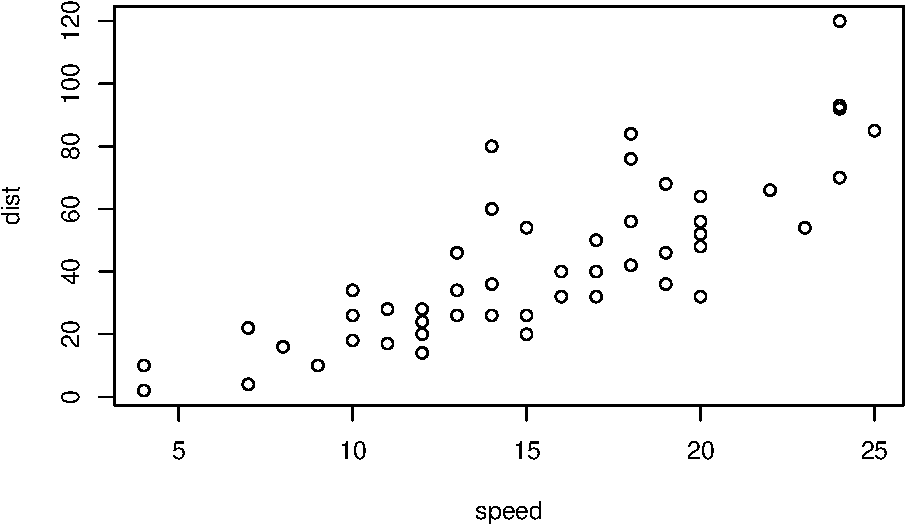
\includegraphics[width=0.8\linewidth]{yihui_mini_files/figure-latex/fig1-1} 

}

\caption{caption}\label{fig:fig1}
\end{figure}

Tab. \ref{tab:tab1} psum dolor sit amet, consectetur adipiscing elit,
sed do eiusmod tempor incididunt ut labore et dolore magna aliqua.

\begin{table}

\caption{\label{tab:tab1}Here is a nice table!}
\centering
\begin{tabular}[t]{rrrrl}
\toprule
Sepal.Length & Sepal.Width & Petal.Length & Petal.Width & Species\\
\midrule
5.1 & 3.5 & 1.4 & 0.2 & setosa\\
4.9 & 3.0 & 1.4 & 0.2 & setosa\\
4.7 & 3.2 & 1.3 & 0.2 & setosa\\
4.6 & 3.1 & 1.5 & 0.2 & setosa\\
5.0 & 3.6 & 1.4 & 0.2 & setosa\\
\addlinespace
5.4 & 3.9 & 1.7 & 0.4 & setosa\\
4.6 & 3.4 & 1.4 & 0.3 & setosa\\
5.0 & 3.4 & 1.5 & 0.2 & setosa\\
4.4 & 2.9 & 1.4 & 0.2 & setosa\\
4.9 & 3.1 & 1.5 & 0.1 & setosa\\
\addlinespace
5.4 & 3.7 & 1.5 & 0.2 & setosa\\
4.8 & 3.4 & 1.6 & 0.2 & setosa\\
4.8 & 3.0 & 1.4 & 0.1 & setosa\\
4.3 & 3.0 & 1.1 & 0.1 & setosa\\
5.8 & 4.0 & 1.2 & 0.2 & setosa\\
\addlinespace
5.7 & 4.4 & 1.5 & 0.4 & setosa\\
5.4 & 3.9 & 1.3 & 0.4 & setosa\\
5.1 & 3.5 & 1.4 & 0.3 & setosa\\
5.7 & 3.8 & 1.7 & 0.3 & setosa\\
5.1 & 3.8 & 1.5 & 0.3 & setosa\\
\bottomrule
\end{tabular}
\end{table}

\section{Conclusions}\label{conclusions}

Lorem ipsum dolor sit amet, consectetur adipiscing elit, sed do eiusmod
tempor incididunt ut labore et dolore magna aliqua. Ut enim ad minim
veniam, quis nostrud exercitation ullamco laboris nisi ut aliquip ex ea
commodo consequat. Duis aute irure dolor in reprehenderit in voluptate
velit esse cillum dolore eu fugiat nulla pariatur. Excepteur sint
occaecat cupidatat non proident, sunt in culpa qui officia deserunt
mollit anim id est laborum

\hypertarget{refs}{}
\hypertarget{ref-chowell2016elucidating}{}
Chowell, Gerardo, Julie M Cleaton, and Cecile Viboud. 2016.
``Elucidating Transmission Patterns from Internet Reports: Ebola and
Middle East Respiratory Syndrome as Case Studies.'' \emph{The Journal of
Infectious Diseases} 214 (suppl\_4). Oxford University Press:
S421--S426.

\hypertarget{ref-liu2016epidms}{}
Liu, Sicong, Silvestro Poccia, K Selçuk Candan, Gerardo Chowell, and
Maria Luisa Sapino. 2016. ``EpiDMS: Data Management and Analytics for
Decision-Making from Epidemic Spread Simulation Ensembles.'' \emph{The
Journal of Infectious Diseases} 214 (suppl\_4). Oxford University Press:
S427--S432.


\end{document}
